\lecture{Master Production Schedule (MPS) e Rough Cut Capacity Planning (RCCP)}{16~-~02~-~2026}
%
\section{Master Production Schedule}
Il Master Production Schedule (MPS) è il cuore della pianificazione operativa. Esso definisce le quantità di ``end-items'' da produrre in specifici intervalli di tempo, derivando tali dati dal Piano di Produzione (Pianificazione Aggregata).

È fondamentale comprendere che l'MPS agisce a livelli diversi della distinta base a seconda della strategia produttiva adottata dall'azienda (il cosiddetto Customer Decoupling Point):
\begin{itemize}
    \item \textbf{Make to Stock} (MTS): Produzione per il magazzino. L'MPS pianifica i prodotti finiti. Si applica a prodotti standardizzati con bassa varietà e domanda prevedibile;
    \item \textbf{Assemble to Order} (ATO): Assemblaggio su ordine. L'MPS pianifica i prodotti intermedi (sotto-assemblati). Permette alta varietà finale partendo da moduli standard (es. automobili);
    \item \textbf{Make to Order} (MTO): Produzione su ordine. L'MPS pianifica le materie prime. Massima personalizzazione, scorte costituite solo da materiali grezzi.
\end{itemize}

%
\subsection{Logica di calcolo}
L'obiettivo primario dell'MPS è mantenere il livello di scorta (Inventory) non negativo, individuando esattamente quando e quanto produrre.

%
\paragraph{Projected On-Hand Inventory} Fornisce una stima delle scorte disponibili in ogni periodo dopo che è stata soddisfatta la domanda di quel periodo.
\[
    I_{t} = I_{t-1}+\mathit{MPS} - \max \left\{ F_{t}, O_{t} \right\}
\]
dove:
\begin{itemize}
    \item $ I_{t} $: previsione disponibilità magazzino nel periodo $ t $, $ I_{t-1} $ è la scorta del periodo precedente;
    \item $ \mathit{MPS} _{t} $: previsione quantità prodotta nel periodo $ t $;
    \item $ F_{t} $: previsione della domanda nel periodo $ t $;
    \item $ O_{t} $: ordini acquistati nel periodo $ t $.
\end{itemize}
Lo scopo dell'$ \mathit{MPS} $ è mantenere non negativo il projected on-hand
inventory individuando quando e quanto produrre.

\begin{note}
    Viene sempre assunto il massimo tra domanda prevista e ordini acquisiti per
    salvaguardare la sicurezza del piano.
\end{note}

%
\paragraph{Available-to-Promise (ATP)} L'ATP indica la quantità di prodotto finito che il reparto vendite può promettere ai clienti senza compromettere gli ordini già acquisiti. È la quota di produzione non ancora ``prenotata''.

\noindent % Impedisce il rientro del primo blocco
\begin{minipage}[t]{0.48\textwidth} % [t] allinea i blocchi in alto
    \subparagraph{Primo periodo}
    \[
        \mathit{ATP}_{1} = I_{0} + \mathit{MPS}^{0}_{1} - \sum_{t'=1}^{\mathit{MPS}^{1}_{t}} O_{t}
    \]
    \small Si considera l'inventario iniziale ($I_{0}$) più l'MPS attuale, sottraendo tutti gli ordini ricevuti fino a quando non verrà rilasciato un nuovo lotto MPS.
\end{minipage}
\hfill
\begin{minipage}[t]{0.48\textwidth}
    \subparagraph{Altri periodi}
    \[
        \mathit{ATP}_{t} = \mathit{MPS}^{0}_{t} - \sum_{t'=t}^{\mathit{MPS}^{1}_{t}} O_{t}
    \]
    \small Qui non si considera più l'inventario pregresso, ma solo la nuova produzione netta rispetto agli ordini coperti da quel lotto.
\end{minipage}

Per entrambi, con $ \mathit{MPS}^{0} $ si intende l'$ \mathit{MPS} $, mentre con $ \mathit{MPS}^{1} $ si intende l'$ \mathit{MPS} $ successivo.

%
\paragraph{Regola di accettazione ordini} Un nuovo ordine può essere accettato solo se la sua quantità non rende negativo l'ATP del periodo richiesto (o riduce eccessivamente l'ATP cumulato, a seconda della logica temporale).

%
\subsection{Congelamento del Piano}
Modificare l'MPS all'ultimo minuto è costoso e rischioso. Per questo si istituiscono delle barriere temporali:
\begin{itemize}
    \item \textbf{Demand Time Fence} (DTF): Periodo ``congelato'' (\emph{frozen}). Nessuna modifica automatica è permessa; ogni cambiamento richiede autorizzazioni speciali poiché siamo vicini alla produzione/consegna.
    \item \textbf{Planning Time Fence} (PTF): Periodo ``slushy''. L'MPS non viene ricalcolato automaticamente dal sistema, ma il pianificatore può intervenire manualmente per aggiustare le quantità (\emph{Firm Planned Orders}).
\end{itemize}

DTF e PTF devono essere controllati ed aggiornati continuamente.

\begin{figure}
    \centering
    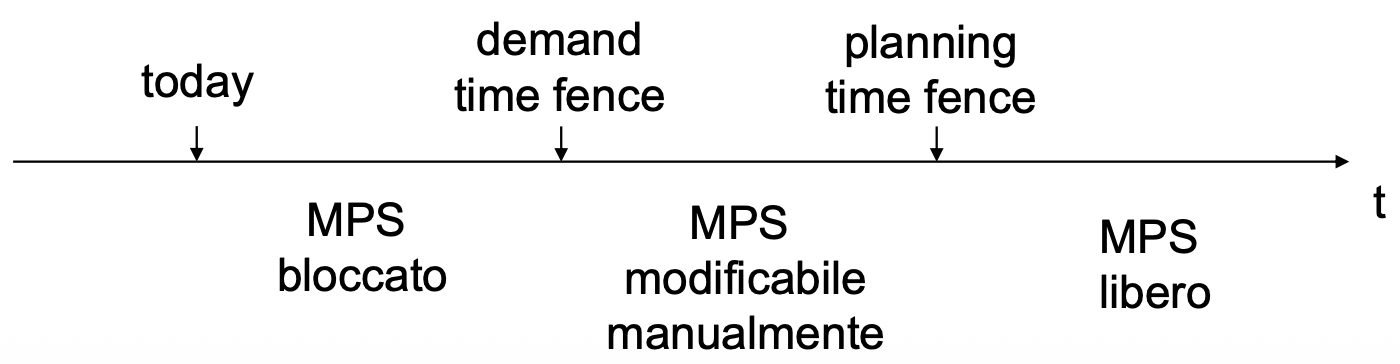
\includegraphics[width=0.7\linewidth]{assets/Screenshot 2026-02-17 at 11.19.12.png}
    \caption{Linea temporale dell'MPS}
\end{figure}

%
\section{Rough Cut Capacity Planning}
L'RCCP è utilizzato per verificare la fattibilità di un MPS controllando il carico di lavoro di alcune risorse critiche. Quest'ultimo utilizza una ``lista delle risorse'' utilizzate da ciascun prodotti finito dell'MPS.

La lista delle risorse (bill of resources o capacity bill) contiene il tempo di processo sulle risorse critiche necessarie alle realizzazione di un prodotto finito.

%
\paragraph{Procedura RCCP}
\noindent \setcounter{step}{0}
\begin{multicols}{2}
    \begin{stepbox}
        Utilizzare la Bill of Resources (Distinta delle Risorse), che indica quante ore di lavoro servono su ogni centro di lavoro critico per produrre una unità di prodotto finito.
    \end{stepbox}
    \begin{stepbox}
        Moltiplicare le quantità dell'MPS per i tempi unitari della Bill of Resources.
    \end{stepbox}
    \begin{stepbox}
        Sommare il carico totale per periodo su ogni Centro di Lavoro (Workstation).
    \end{stepbox}
    \begin{stepbox}
        Confrontare il carico totale con la capacità disponibile (rappresentata spesso da una linea rossa nei grafici, es. 3000 ore).

        I grafici sono con $ x = \text{Time}, \quad y = \text{Workload} $
    \end{stepbox}
\end{multicols}